\documentclass[12pt, a4paper, lithuanian]{article}
\usepackage[utf8x]{inputenc}
\def\LTfontencoding{L7x}
\PrerenderUnicode{ąčęėįšųūž}
\usepackage[\LTfontencoding]{fontenc}
\usepackage[lithuanian]{babel}
\usepackage{VUMIFCS1bakalaurinis}
\usepackage{cite}
\usepackage{amsmath}
\usepackage{bm}
\usepackage{amsfonts}
\usepackage{float}
\usepackage{graphicx}
\usepackage{color}
\usepackage{listings}
\usepackage{wrapfig}
\usepackage{algpseudocode}
\usepackage{algorithm}
\usepackage{algorithmicx}
\usepackage{caption}
\usepackage{subfig}


% Titulinio aprašas
\vumifdept{Informatikos katedra}
\vumifpaper{Baigiamasis bakalauro darbas}
\title{Rizikų valdymo proceso modeliavimas}
\titleineng{Modeling of Risk Management Process}
\status{2 kurso 1 grupės studentas}
\author{Vardenis Pavardenis}
% \secondauthor{Vardonis Pavardonis}
\supervisor{doc. dr. Vardaitis Pavardaitis}
\reviewer{dr. Vardauskas Pavardauskas}
\date{Vilnius\\ \the\year}

\begin{document}
\maketitle

\tableofcontents

\sectionnonum{Įvadas}
...

\section{RPC mechanizmas}
... citavimo pavyzdys \cite{Banerjee1997}, \cite{EgArticle} ...

\subsection{Kliento-serverio modelis}
\subsection{Serverio-skaičiuotojo modelis}
\subsection{Kaip dirba RPC}

\section{Programų, naudojančių RPC, kūrimas}
\subsection{Kūrimo etapai}
\subsubsection{RPC SDK instaliavimas}
\subsubsection{Detalaus programų sistemų projektavimas}
\subsubsection{Objektinių modulių ryšių redagavimas}
\subsection{IDL failas}
\subsubsection{IDL failo antraštė}
\subsubsubsection{Atributas "`uuid"'}
\subsubsubsection{Atributas "`version"'}
\subsubsubsection{Atributas "`local"'}
\subsubsection{IDL failo kūnas}
\subsubsubsection{Baziniai tipai}
\subsubsubsection{Direktyva "`import"'}
\subsubsubsection{Funkcijų deklaracijos}
\subsection{ACL failas}
\subsubsection{ACF failo antraštė}
\subsection{MIDL kompiliatoriaus generuojami failai}
\section{RPC panaudojimo pavyzdys}
\subsection{Problemos formulavimas}
\subsection{Užduotis}
\subsubsection{Pradiniai reikalavimai}
\subsection{Analizė}
\subsubsection{RS-232}
\subsubsection{Vardiniai kanalai}
\subsubsection{Oracle}
\subsubsection{RPC}
\subsection{Realizacija}
\subsubsection{Registracija}
\subsubsection{Diskusija}

\sectionnonum{Išvados}
...

\bibliography{bibliografija}

\appendix

\section{Niauroninio tinklo struktūra}
\begin{figure}[H]
    \centering
    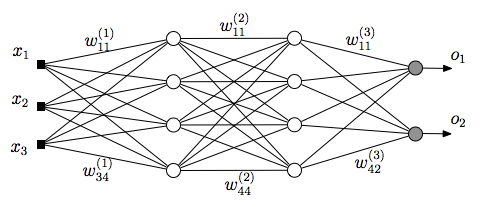
\includegraphics[scale=0.5]{img/MLP}
    \caption{Paveikslėlio pavyzdys}
    \label{img:mlp}
\end{figure}


\section{Eksperimentinio palyginimo rezultatai}
% tablesgenerator.com - converts calculators, e.g. excel, tables to LaTeX
\begin{table}[H]\footnotesize
  \centering
  \caption{Lentelės pavyzdys.}
  {\begin{tabular}{|l|c|c|} \hline
    Algoritmas & $\bar{x}$ & $\sigma^{2}$ \\
    \hline
    Algoritmas A  & 1.6335    & 0.5584       \\
    Algoritmas B  & 1.7395    & 0.5647       \\
    \hline
  \end{tabular}}
  \label{tab:table example}
\end{table}

\end{document}
